\chapter{Casi D'uso}\label{casiDuso}
\section{Attori dei casi d'uso}
\begin{center}
	\begin{figure}[H]
		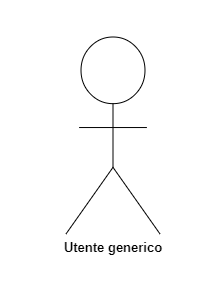
\includegraphics{../immagini/attori_casi/attore.png}
		\caption{Attore: utente generico}
	\end{figure}
\end{center}
\subsection{Attori Primari}\label{attoriPrimari}
\begin{itemize}
	\item \textbf{Utente generico:} Definisce l'utente generico che utilizza l'applicazione web;
	\item \textbf{Fonti esterne:} Definisce le fonti da cui verranno elaborati e visualizzati i dati.
\end{itemize}

\section{Elenco casi d'uso}\label{elencoCasiDuso}
In questa sezione vengono elencati i casi d'uso individuati per il progetto GDP in accordo con il proponente. Ogni caso d'uso indica un'interazione tra uno o più attori e il sistema. Questa interazione genera uno scenario che è l'insieme delle azioni che hanno in comune uno scopo finale per un utente.

\subsection{Azioni dell'utente}
%qui andrebbe il primo diagramma disegnato%
\begin{itemize}
	\item \textbf{Attori primari}: utente generico;
	\item \textbf{Descrizione}: l'utente può decidere che città visualizzare e la tipologia di dati legati ad essa;
	\item \textbf{Scenario principale}: è presente un elemento per far selezionare all'utente la città e la tipologia di dati da visualizzare;
	\item \textbf{Precondizione}: il sistema è attivo e funzionante;
	\item \textbf{Postcondizione}: il sistema fa cose e l'utente vede ciò che ha richiesto.
\end{itemize}

\subsection{UC1 - Scelta della città}
\begin{itemize}
\item \textbf{Attori primari}: utente generico;
\item \textbf{Descrizione}: l'utente può decidere che città visualizzare;
\item \textbf{Scenario principale}: è presente un elemento per far selezionare all'utente la città;
\item \textbf{Precondizione}: il sistema è attivo e funzionante;
\item \textbf{Postcondizione}: il sistema fa cose e l'utente vede ciò che ha richiesto.
\end{itemize}

\subsection{UC2 - Scelta della tipologia dei dati}
\begin{itemize}
	\item \textbf{Attori primari}: utente generico;
\item \textbf{Descrizione}: l'utente sceglie la tipologia di dati disponibili da rappresentare nella mappa;
\item \textbf{Scenario principale}: l'utente accede all'applicazione web e seleziona il tipo di dato da visualizzare. Il sistema fornisce i dati alla mappa e viene così aggiornata;
\item \textbf{Estensione}: 
\begin{itemize}
	\item \textbf{UC3}: se l'applicazione web non riceve nessuna informazione dal sistema viene visualizzato un messaggio di errore.
\end{itemize}
\item \textbf{Precondizione}: il sistema è attivo e funzionante e l'utente sceglie la tipologia di dati da utilizzare;
\item \textbf{Postcondizione}: il sistema invia i dati all'applicazione web e aggiorna la mappa in base alle nuove informazioni.
\end{itemize}

\subsection{UC2.1 - Scelta visualizzazione dati in tempo reale}
\begin{itemize}
	\item \textbf{Attori primari}: utente generico;
	\item \textbf{Descrizione}: l'utente sceglie la tipologia dati in tempo reale da rappresentare nella mappa;
	\item \textbf{Scenario principale}: l'utente accede all'applicazione web e seleziona la visualizzazione dati in tempo reale. Il sistema fornisce solo i dati richiesti alla mappa e viene così aggiornata;
	\item \textbf{Precondizione}: il sistema è attivo e funzionante e i dati in tempo reale sono presenti nel sistema;
	\item \textbf{Postcondizione}: il sistema invia i dati in tempo reale all'applicazione web e aggiorna la mappa in base alle nuove informazioni.
\end{itemize}

\subsection{UC2.2 - Scelta visualizzazione dati storici}
\begin{itemize}
	\item \textbf{Attori primari}: utente generico;
	\item \textbf{Descrizione}: l'utente sceglie la tipologia dati storici da rappresentare nella mappa;
	\item \textbf{Scenario principale}: l'utente accede all'applicazione web e seleziona la visualizzazione dati storici. Il sistema fornisce solo i dati richiesti alla mappa e viene così aggiornata;
	\item \textbf{Precondizione}: il sistema è attivo e funzionante e i dati storici sono presenti nel sistema;
	\item \textbf{Postcondizione}: il sistema invia i dati storici all'applicazione web e aggiorna la mappa in base alle nuove informazioni.
\end{itemize}

\subsection{UC2.3 - Scelta visualizzazione dati predetti}
\begin{itemize}
	\item \textbf{Attori primari}: utente generico;
	\item \textbf{Descrizione}: l'utente sceglie la tipologia dati con predizione da rappresentare nella mappa;
	\item \textbf{Scenario principale}: l'utente accede all'applicazione web e seleziona la visualizzazione dati con predizione. Il sistema fornisce solo i dati richiesti alla mappa e viene così aggiornata;
	\item \textbf{Precondizione}: il sistema è attivo e funzionante e i dati elaborati dal modello di \textit{machine learning} sono presenti nel sistema;
	\item \textbf{Postcondizione}: il sistema invia i dati predetti all'applicazione web e aggiorna la mappa in base alle nuove informazioni.
\end{itemize}

\subsection{UC3 - Visualizza errore mancanza dati}
\begin{itemize}
	\item \textbf{Attori primari}: utente generico;
	\item \textbf{Descrizione}: l'utente visualizza un messaggio di errore in quanto vi è una mancanza di dati dal sistema;
	\item \textbf{Scenario principale}: l'utente dopo essere entrato nell'applicazione web, seleziona un tipologia di dati da visualizzare nella mappa e il sistema non riesce a completare la richiesta;
	\item \textbf{Precondizione}: i dati richiesti non sono presenti nel sistema;
	\item \textbf{Postcondizione}: il sistema invia un messaggio di errore per informare l'utente che i dati richiesti non sono disponibili.
\end{itemize}

\subsection{Azioni del sistema}
%diagramma GDP%
\begin{itemize}
\item \textbf{Attori primari}: fonti esterne;
\item \textbf{Descrizione}: ;
\item \textbf{Scenario principale}: ;
\item \textbf{Precondizione}: ;
\item \textbf{Postcondizione}: .
\end{itemize}

\subsection{UC4 - Acquisizione dei dati}
%nessun diagramma%
\begin{itemize}
\item \textbf{Attori primari}: fonti esterne;
\item \textbf{Descrizione}: ;
\item \textbf{Scenario principale}: ;
\item \textbf{Precondizione}: ;
\item \textbf{Postcondizione}: .
\end{itemize}

\subsection{UC5 - Errore nell'acquisizione dei dati}
%nessun diagramma%
\begin{itemize}
\item \textbf{Attori primari}: fonti esterne;
\item \textbf{Descrizione}: ;
\item \textbf{Scenario principale}: ;
\item \textbf{Precondizione}: ;
\item \textbf{Postcondizione}: .
\end{itemize}

\subsection{UC6 - Elaborazione dati}
%diagramma uc6%
\begin{itemize}
	\item \textbf{Attori primari}: fonti esterne;
	\item \textbf{Descrizione}: ;
	\item \textbf{Scenario principale}: ;
	\item \textbf{Precondizione}: ;
	\item \textbf{Postcondizione}: .
\end{itemize}

\subsection{UC6.1 - Elaborazione per la predizione dei dati}
%nessun diagramma%
\begin{itemize}
	\item \textbf{Attori primari}: fonti esterne;
	\item \textbf{Descrizione}: ;
	\item \textbf{Scenario principale}: ;
	\item \textbf{Precondizione}: ;
	\item \textbf{Postcondizione}: .
\end{itemize}

\subsection{UC6.2 - Elaborazione per la visualizzazione dei dati}
%nessun diagramma%
\begin{itemize}
	\item \textbf{Attori primari}: fonti esterne;
	\item \textbf{Descrizione}: ;
	\item \textbf{Scenario principale}: ;
	\item \textbf{Precondizione}: ;
	\item \textbf{Postcondizione}: .
\end{itemize}

\subsection{UC7 - Errore nell'elaborazione dati}
%nessun diagramma%
\begin{itemize}
	\item \textbf{Attori primari}: fonti esterne;
	\item \textbf{Descrizione}: ;
	\item \textbf{Scenario principale}: ;
	\item \textbf{Precondizione}: ;
	\item \textbf{Postcondizione}: .
\end{itemize}


%%DA QUI CI SONO LE COSE FATTE DA CECHCIN%%
\subsection{UC1 - Visualizzazione mappa}
\begin{center}
	\begin{figure}[H]
		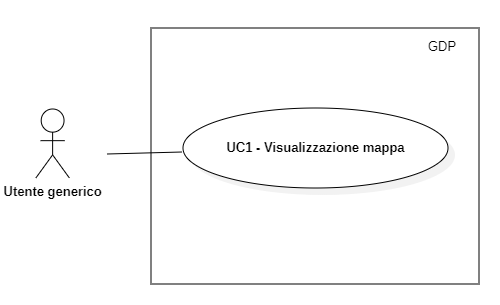
\includegraphics[width=0.95\linewidth]{../immagini/attori_casi/vis_mappa.png}
		\caption{UC1 - Visualizzazione mappa}
	\end{figure}
\end{center}
\begin{itemize}
	\item \textbf{Attori primari}: utente generico;
	\item \textbf{Descrizione}: l'utente visualizza una mappa presente nell'applicazione web. Tale mappa è una heat map e presenta all'utente i dati analizzati dal prodotto;
	\item \textbf{Scenario principale}: l'utente accede all'applicazione web e visualizza la mappa;
	\item \textbf{Precondizione}: il sistema è attivo e funzionante;
	\item \textbf{Postcondizione}: il sistema invia i dati alla pagina al caricamento presentando una mappa con tutti i dati per l'utente.
\end{itemize}
\begin{center}
	\begin{figure}[H]
		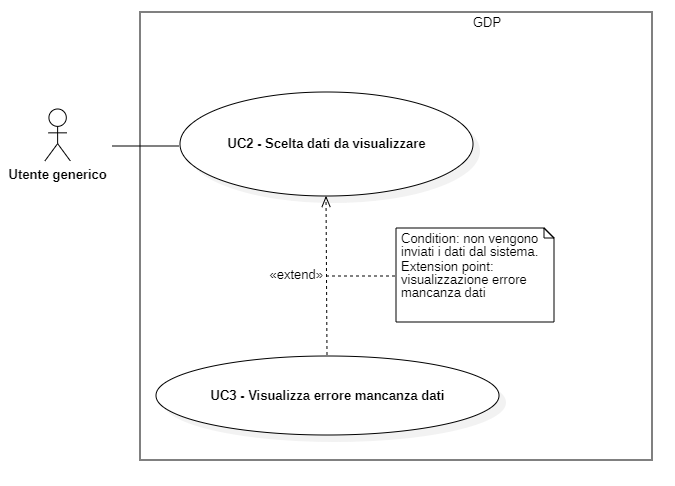
\includegraphics[width=0.95\linewidth]{../immagini/attori_casi/uc2.png}
		\caption{Schema generale: Scelta dati da visualizzare ed errori}
	\end{figure}
\end{center}


